\chapter{Introduction}
\label{ch:introduction}

\section{Motivation}
  Recent interest in advanced and next-generation nuclear power reactor designs
  has encouraged further development of modeling and simulation methods for
  these reactors. Fast reactors, a class of advanced reactors, operate with
  predominately high-energy (``fast'') neutrons in the fission reaction. Since
  early development of fast reactors, such as  \gls{ebr-i} in 1951 and Fermi 1
  in 1956, there have been significant innovations in both nuclear modeling and
  computational methods. As development of fast reactors is revisited in the
  form of the \gls{vtr} at \gls{inl}, improvements in simulation can be
  used to simulate fast reactors with modern best practices. 
  

  Nuclear reactor simulations are inherently multiphysics simulations. For
  example, neutron reaction probabilities are described by cross sections.
  Neutron cross sections are dependent on material temperatures and densities,
  both of which vary over the operating range of a nuclear power reactor. As
  reactor power changes, material temperatures and densities change, therefore
  cross sections change and affect the reactor power. The multiphysics nature
  of the reactor necessitate a simulation of the power distribution within the
  reactor as well as all feedback effects which will be modeled. 
  
  In this thesis, models for simulating fast reactors will be developed and
  demonstrated. Reactor power distribution will be modeled according to the
  multigroup neutron diffusion equation as solved by the \gls{fem} based on
  unstructured meshes with special attention to hexagonal geometries.
  The multigroup neutron diffusion solution method is verified through
  comparison to both benchmark and analytic solutions. Multiphysics effects are
  modeled including thermal hydraulics and thermal expansion. Thermal hydraulic
  effects are modeled as axial heat convection and radial heat conduction.
  Thermal expansion is modeled using simplified linear expansion models. The
  methods developed in this work can easily be used for fast reactors with a
  variety of coolants including sodium, lead, or molten salt.

  By employing a modern solution method to the neutron diffusion equation in the
  form of the \gls{fem}, the simulation can take advantage of developments in
  numerical methods including the solution of linear systems. Additionally, the
  simulation allows for the incorporation of generalized multiphysics effects
  whereas current state-of-the-art techniques (such as \dif) require data
  processing and manual iteration to simulate multiphysics effects. Ultimately, 
  the simulation is designed to simulate an operating fast reactor and estimate
  feedback coefficients by coupling multiphysics models.

\section{Geometry Description}
  \label{sec:geometry_description}
  The high-energy neutron spectra inherent to fast reactors results in
  relatively small neutron cross sections compared to larger cross sections in
  the thermal energy range. To compensate for this fact, fast reactors are
  typically designed with hexagonal, triangularly pitched, fuel assemblies to
  maximize fuel packing. An example of a fast reactor with hexagonal fuel
  assemblies is shown in \fref{fig:reactor_materials}.
  
  \begin{figure}
    \centering
    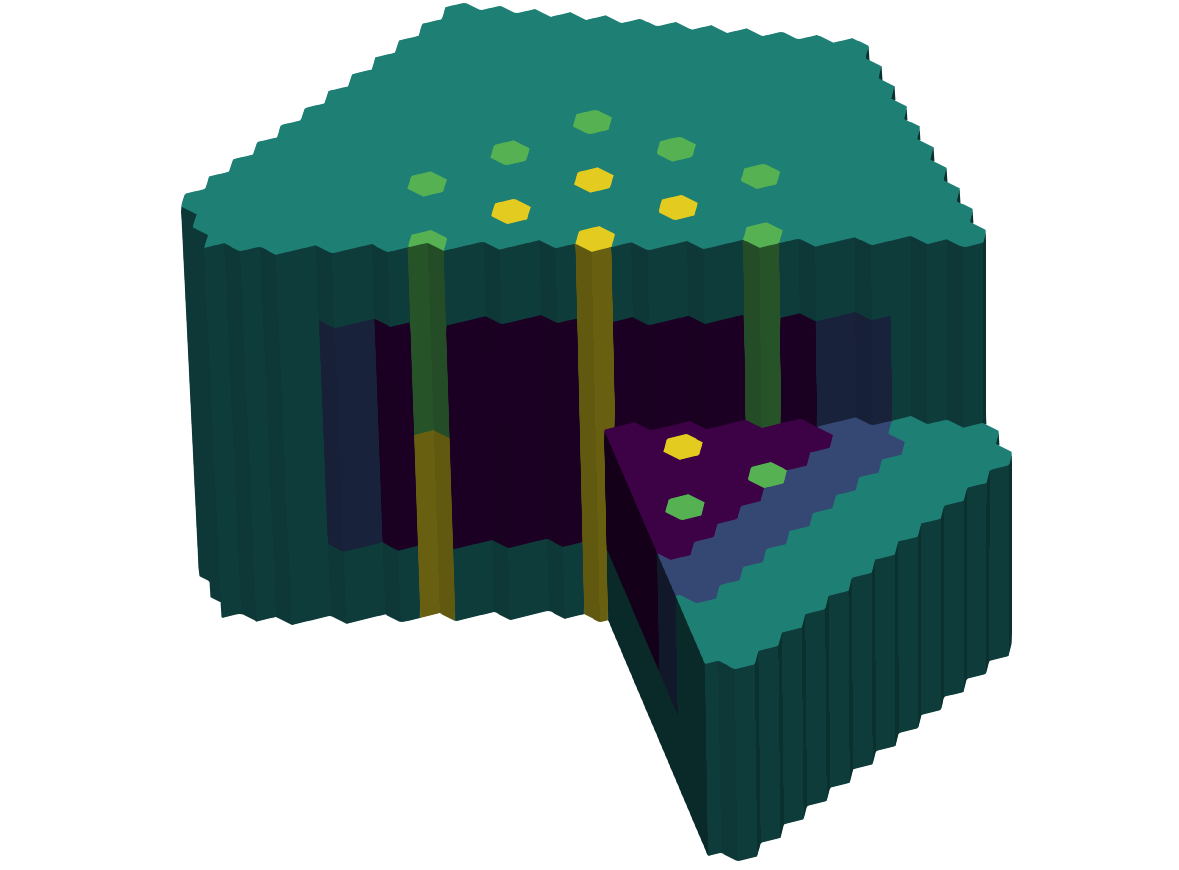
\includegraphics[width=\textwidth]{reactor_materials}
    \caption{Example of Fast Reactor Materials based on MONJU.}
    \label{fig:reactor_materials}
  \end{figure}

  \begin{figure}
    \centering
    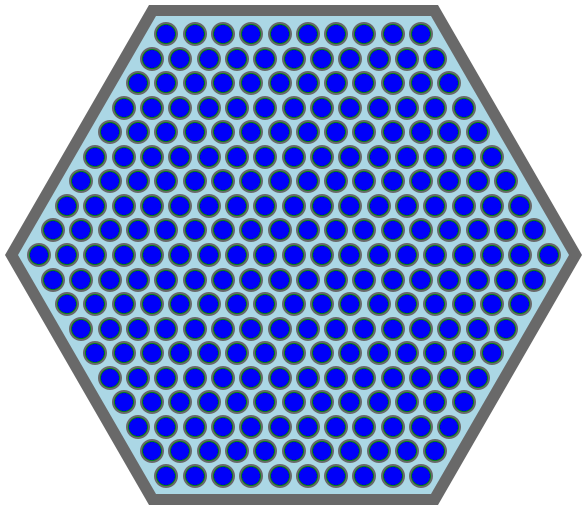
\includegraphics[width=0.5\textwidth]{prism_hex}
    \caption{Example of Fast Reactor Fuel Assembly Cross Section.}
    \label{fig:prism_hex}
  \end{figure}

  A cross-sectional representation of a hexagonal fuel assembly is shown in
  \fref{fig:prism_hex}. This geometry is used in the homogenization of neutron
  cross sections and is also used to describe coolant flow geometries.
  Dimensions of assemblies are measured at room temperature and will later be
  expanded according to the thermal expansion model in
  \chref{ch:thermalExpansion}.

  Note the individual rods in \fref{fig:prism_hex} are cylindrical and are
  arranged into a hexagonal assembly. The basic geometry is a metallic fuel
  material within stainless steel cladding. The gap between the fuel and
  cladding is filled by sodium bond to improve thermal conductivity across the
  gap. The rod is helically wrapped by a steel wire to ensure separation between
  rods that will allow for coolant flow. The wire wrap also serves to encourage
  the mixture of coolant within the assembly. (Note: wire wrap is omitted from
  \fref{fig:prism_hex}.) Many rods are then assembled into an assembly and
  surrounded by a hexagonal can made of steel. This can aids in structural
  stability and prohibits cross-flow of coolant between assemblies. 

  The dimensions within a single rod are shown in \fref{fig:pin_model} and the
  dimensions within a hexagonal assembly can are shown in \fref{fig:hex_can}. In
  \fref{fig:hex_can}, $T\!h_{can}$ is the thickness of the assembly can,
  $F\!2\!F$ is the flat-to-flat measurement of the outside of the hexagonal can,
  and \textit{Pitch} is the distance between the center of two rods. Using the
  geometry described in these figures, the material cross-sectional areas are
  calculated according to the given formulae where $N_{rod}$ is the number of
  rods in the assembly and $A\!P$ is the assembly pitch. $A\!P > F\!2\!F$ to
  account for inter-assembly sodium gaps (see ``Gap'' in \fref{fig:hex_can}).
  \begin{align}
    \label{eq:afrac_first}
    A_{total} &= \frac{\sqrt{3}}{2} A\!P^2 \\
    A_{box} &= 
      \frac{\sqrt{3}}{2} \left(F\!2\!F^2 - \left(F\!2\!F - 2
      Th_{can}\right)^2\right) \\
    A_{wrap} &= N_{rod} \frac{\pi}{4} D_{wrap}^2 \\
    A_{clad} &= N_{rod} \pi (R_C^2 - R_B^2) \\
    A_{bond} &= N_{rod} \pi (R_B^2 - R_F^2) \\
    A_{fuel} &= N_{rod} \pi R_F^2 \\
    A_{cool} &= A_{total} - A_{box} - A_{wrap} - A_{clad} - A_{bond} -
      A_{fuel}\\
    \label{eq:afrac_last}
    A_{struct} &= A_{box} + A_{wrap} + A_{clad}
  \end{align}
  Calculating the areas as above allows for calculation of cross-sectional area
  fractions. Assuming constant dimensions in the axial direction, these area
  fractions are equivalent to volume fractions and are useful for neutron
  cross section homogenization. Additionally, these formulae allow for thermal
  expansion as the liquid sodium in the bond and the liquid coolant are allowed
  to vary to allow for the expansion of other materials.

  \begin{figure}
    \centering
    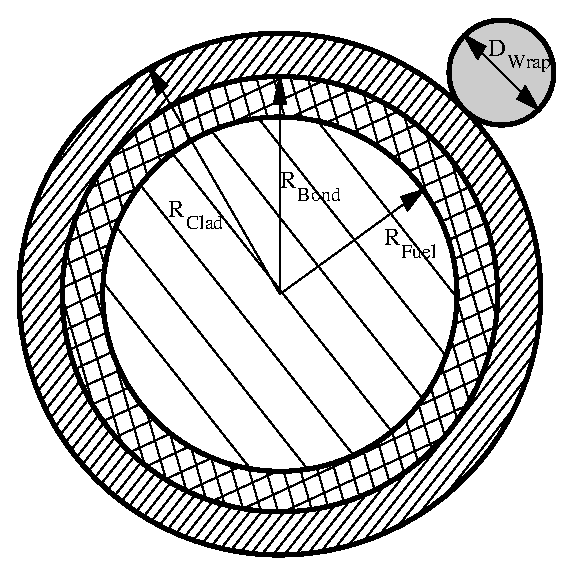
\includegraphics[width=0.5\textwidth]{pin_model}
    \caption{Dimensions of Thermal Hydraulic Rod Model (not to scale).}
    \label{fig:pin_model}
  \end{figure}

  \begin{figure}
    \centering
    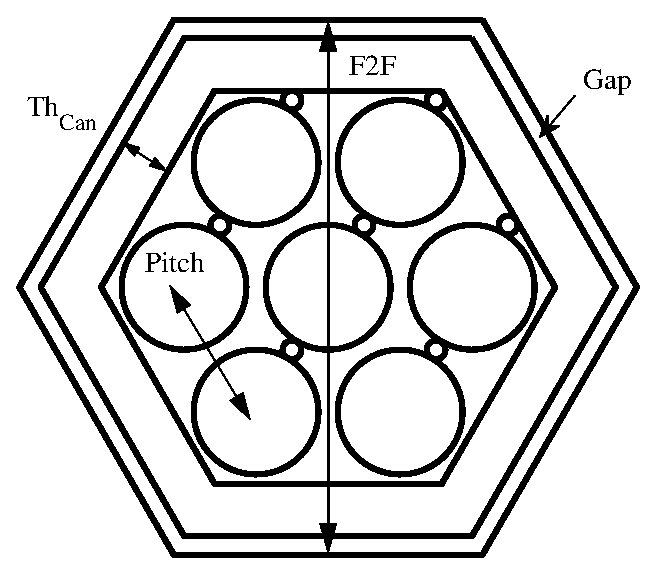
\includegraphics[width=0.5\textwidth]{hex_can}
    \caption{Dimensions of Hexagonal Can (not to scale).}
    \label{fig:hex_can}
  \end{figure}

\section{Cross Section Treatment}
  \label{sec:cross_section_treatment}
  Reactor materials are ``smeared'' into homogeneous regions. This treatment is
  common to fast reactors because of the relatively large neutron
  mean-free-paths compared to the scale of material dimensions. Additionally,
  the neutron distribution will be modeled using the neutron diffusion equation
  which cannot accurately resolve small geometric details. The natural
  choice for these homogeneous regions are the hexagonal assemblies themselves.
  Materials are permitted to be heterogeneous axially. For this work, four
  distinct regions are modeled within a hexagonal assembly: fuel, bond, coolant,
  and steel. Steel material includes cladding, wire wrap, and assembly can. 
  These four regions are then homogenized into a hexagonal assembly.

  For simplified analytic and benchmark problems, cross sections are specified
  by the problem. For realistic simulations, multigroup microscopic cross
  sections are generated using the computer program \mcc \cite{mcc}. The cross
  section generator uses 2,082 fine energy groups to collapse down to an
  arbitrary number of coarse energy groups. For this simulation, the recommended
  and default 33-group energy structure is used. However, the methods in this
  work are implemented generally and are not dependent on a particular energy
  group structure. \mcc solves the infinite-homogeneous (zero-dimension) neutron
  transport equation for isotopic number densities as input by the user.  Cross
  sections for each assembly type are generated separately to accurately
  simulate the neutron energy spectrum within the assembly. This procedure
  results in a unique material cross sections for each assembly type. For
  example, each assembly type contains steel; therefore, there will be a
  separate steel cross section for each assembly type in the cross section
  library. Within \mcc, the neutron energy spectrum for fissile media is
  generated by the media's fission spectrum.  Non-fissile homogenized mixtures,
  such as control assemblies or reflector assemblies, the default
  \isotope[238]{U} fission spectrum is assumed.

  Cross section libraries are generated for several different temperatures to
  capture temperature-dependent cross section effects. These libraries are then
  used during the simulation to calculate cross sections as a function of
  material temperatures. The fuel, clad, and coolant temperatures in a
  simulated reactor can be calculated with a thermal hydraulic model (see
  \chref{ch:thermalHydraulics}). However, the temperatures calculated in the
  thermal hydraulic model are functions of reactor power and coolant mass flow
  rate. These parameters are not known before the simulation for a general
  reactor. Instead, a simplified one-dimensional, single-channel model is used
  to estimate temperatures for cross section library generation. This model is
  based on the axial convection and radial conduction models in
  \chref{ch:thermalHydraulics}. The simulation model can use general cross
  section library temperatures and a general number of temperature libraries.
  A user may select the number of cross section libraries and specify the
  temperatures for which the libraries apply in a general manner. Typical 
  cross section library temperatures for simulating liquid metal cooled, metal
  fueled, fast reactors are given in \tref{tab:xstemps}.

  \begin{table}
    \caption{Temperatures Selected for Cross Section Libraries.}
    \label{tab:xstemps}
    \begin{center}
      \begin{tabular}{crrr}
        \toprule
        Library & $T_{cool} \units{K}$ & $T_{clad} \units{K}$ & 
          $T_{fuel} \units{K}$ \\
        \midrule
        1 & 628.15 & 628.15 & 628.15  \\
        2 & 708.65 & 757.50 & 807.15  \\
        3 & 896.87 & 920.47 & 961.46 \\
        4 & 1072.81 & 1114.83 & 1183.14 \\
        \bottomrule
      \end{tabular}
    \end{center}
  \end{table}

  Note that the maximum temperatures in \tref{tab:xstemps} are greater than 
  temperatures observed at typical reactor operating conditions. This is
  necessary so that even at perturbed reactor conditions (e.g. $110\%$ full
  power), the peak core temperatures can still be interpolated within the
  libraries.

  Cross sections are homogenized within each hexagonal assembly using isotopic
  microscopic cross sections from \mcc and user input number densities.
  Homogenization is performed in two steps: first, isotopic homogenization and
  second, volumetric homogenization. Isotopic homogenization is performed by
  summing microscopic cross sections and associated number densities. Let
  $\sigma_{i,j,x,g}$ represent the microscopic cross section for isotope $i$, in
  region $j$, for reaction type $x$, and energy group $g$ as output by \mcc.
  $\sigma_{i,j,x,g}$ has units of area. Then, let $N_{i,j}$ represent the atom
  number density for isotope $i$ in region $j$ as input by the user. $N_{i,j}$
  has units of inverse volume. The macroscopic cross section can then be
  defined
  \begin{equation}
    \label{eq:isotopic_homogenization}
    \Sigma_{j,x,g} = \sum_{i=1}^{N_{iso}} N_{i,j} \, \sigma_{i,j,x,g}
  \end{equation}
  where $\Sigma_{j,x,g}$ is the macroscopic cross section in region $j$, for
  reaction type $x$, and energy group $g$. In \eref{eq:isotopic_homogenization},
  $N_{iso}$ represents the number of isotopes in region $j$. Note that
  $\Sigma_{j,x,g}$ will have units of inverse length.

  Next, volumetric cross section homogenization is performed using volume
  fractions. Assuming dimensions do not change axially within a hexagonal
  assembly, the areas calculated in \eref{eq:afrac_first} through
  \eref{eq:afrac_last} can be used to calculate area fractions.
  These area fractions can subsequently be treated as volume fractions.
  Using the definition of macroscopic cross sections from
  \eref{eq:isotopic_homogenization}, the volumetrically homogenized macroscopic
  cross section is 
  \begin{equation}
    \label{eq:volumetric_homogenization}
    \Sigma_{x,g} = \frac{\sum_{j = 1}^{N_{reg}} \Sigma_{j,x,g} \, V_j}
      {\sum_{j=1}^{N_{reg}} V_j}
  \end{equation}
  where $V_j$ is the volume or area occupied by region $j$ in the hexagonal
  assembly and $N_{reg}$ is the number of regions in the hexagonal assembly.
  Typically, $N_{reg} = 4$ with unique regions for fuel, sodium bond, sodium
  coolant, and steel structural material. After homogenizing cross sections
  isotopically and volumetrically, the diffusion coefficient for energy group
  $g$, $D_g$, can be calculated as 
  \begin{equation}
    \label{eq:diffusion_homogenization}
    D_g = \frac{1}{3 \Sigma_{tr,g}}
  \end{equation}
  where $\Sigma_{tr,g}$ represents the macroscopic transport cross section for
  energy group $g$. $\Sigma_{tr,g}$ has been homogenized according to
  \eref{eq:isotopic_homogenization} and \eref{eq:volumetric_homogenization}.
  Note that $D_g$ will have units of length.

\section{Thesis Organization}
  In \chref{ch:neutronDiffusion}, the derivation of the \gls{fem} solution to
  the multigroup neutron diffusion equation is presented. Special attention is
  paid to triangular and wedge elements. The resulting eigenvalue problem is
  solved using the Power Method. Results from the diffusion solution are
  verified in two-dimensional and three-dimensional problems with both analytic 
  and benchmark solutions. These verification problems for the neutron diffusion
  equation are presented in \chref{ch:diffusionResults}.

  \chref{ch:thermalHydraulics} presents the formulation of axial heat convection
  and radial heat conduction models for a typical fast reactor. These models are 
  used to calculate material temperatures and update cross sections for the 
  simulation. Results of the numerical model are compared to analytical models 
  and example material temperatures are shown.

  In \chref{ch:thermalExpansion} a simplified thermal expansion model is
  presented. The model assumes linear thermal expansion for given material
  properties and user-specified thermal expansion temperatures. A simple
  demonstration of the effects of thermal expansion on reactivity are presented.

  The combination of all of these models allows for the realistic simulation of
  a fast reactor. In \chref{ch:coupledResults}, the multiphysics models are
  coupled and investigated for a benchmark reactor problem. Using this benchmark
  reactor and the models described, multiphysics reactivity feedback
  coefficients are estimated.
 
  Finally, \chref{ch:conclusions} presents a summary and the conclusions of this
  research. Additionally, recommendations for further research are provided.
